\documentclass[journal]{IEEEtran}

%%%% Using Latex Packages %%%%


\usepackage{cite}
\usepackage{amsmath,amssymb,amsfonts}
\usepackage{algorithmic}
\usepackage{subcaption}
\usepackage{color}
\usepackage{graphicx}
\usepackage{xcolor}
\usepackage{enumerate}
\usepackage{multirow}
\usepackage{amsmath}
\usepackage{amssymb}
\usepackage[utf8]{inputenc}
\usepackage[ruled]{algorithm2e}
\usepackage[colorinlistoftodos]{todonotes}
\def\BibTeX{{\rm B\kern-.05em{\sc i\kern-.025em b}\kern-.08em
    T\kern-.1667em\lower.7ex\hbox{E}\kern-.125emX}}
\newtheorem{definition}{Definition}
\renewcommand{\topfraction}{1.0}
\renewcommand{\bottomfraction}{1.0}
\renewcommand{\dbltopfraction}{1.0}
\renewcommand{\textfraction}{0.01}
\renewcommand{\floatpagefraction}{1.0}
\renewcommand{\dblfloatpagefraction}{1.0}
\setcounter{topnumber}{5}
\setcounter{bottomnumber}{5}
\setcounter{totalnumber}{10}


\hyphenation{op-tical net-works semi-conduc-tor}


\begin{document}

\title{Efficient Feasibility Checking Algorithm of Photovoltaic Array Reconfiguration}

\author{Dafang Zhao,
        Fukohito Ooshita,~\IEEEmembership{Member,~IEEE}
        and~Michiko~Inoue,~\IEEEmembership{Member,~IEEE}}% <-this % stops a space

% \thanks{M. Shell was with the Department
% of Electrical and Computer Engineering, Georgia Institute of Technology, Atlanta,
% GA, 30332 USA e-mail: (see http://www.michaelshell.org/contact.html).}% <-this % stops a space
% \thanks{J. Doe and J. Doe are with Anonymous University.}% <-this % stops a space
% \thanks{Manuscript received April 19, 2005; revised August 26, 2015.}}

% note the % following the last \IEEEmembership and also \thanks - 
% these prevent an unwanted space from occurring between the last author name
% and the end of the author line. i.e., if you had this:
% 
% \author{....lastname \thanks{...} \thanks{...} }
%                     ^------------^------------^----Do not want these spaces!


% make the title area
\maketitle

% As a general rule, do not put math, special symbols or citations
% in the abstract or keywords.
\begin{abstract}
  Power generation efficiency of photovoltaic (PV) systems is significantly affected buy partial shading and PV cell damage.
  Partial shading or PV cell damage induces mismatched power generation among PV panels.
  Conducted bypass diodes under mismatch conditions result in loss of efficiency in power generation.
  Mismatched PV array can be recovered by re-configuring electrical connections among PV panels in it.
  In this paper, a feasibility check problem of PV panel reconfiguration is introduced.
  This problem identifies whether a connection among PV panels can be configured from a given PV module level solution.
  Proposed algorithm evaluated by comparison with the exhaustive search through random shading distributed PV array.
  The experimental results demonstrate that proposed algorithm can identify feasible configurations more than 49,000 times faster than the exhaustive search with around 0.5\% errors.
\end{abstract}

% Note that keywords are not normally used for peerreview papers.
\begin{IEEEkeywords}
PV reconfiguration, partial-shading, mismatch, feasibility, heuristic
\end{IEEEkeywords}

\IEEEpeerreviewmaketitle



\section{Introduction}
\IEEEPARstart{I}{n} recent years, the use of green and renewable energy sources has been increased with the aim to reduce fossil fuel depletion and environment pollution.
Photovoltaic (PV) energy is one of the most promising emerging technologies.
PV market growth by improvements of converting unlimited solar energy into electrical energy as well as the cost reductions of PV panels.

The use of PV systems for power generation brings many challenges.
Due to the nature of PV cell, which is the basic component of PV array.
PV system easily suffers from various forms of system faults, which include physical damage, temperature in-homogeneity, or partial shading.
Unlike cell damage or other system faults, partial shading sources from cloud, dust or snow are very hard to prevent and predict.
Thus, when PV cell could not uniformly generate power when they experience different irradiance or been damaged.
This unbalanced working scenario will lead whole system mismatch.
Mismatch condition might accelerate heating or aging of PV cells and furthermore hinder operation of maximum power point tracking (MPPT) algorithm, especially when the PV array output P-V curve becomes non-convex\cite{islam2018performance}.

For several series connected PV cells, shaded or damaged cell causing normal cells to produce higher voltages that may reverse bias of ``bad'' cells.
When a large number of series connected cells cause a huge reverse bias across shaded cells, leading to large dissipation of energy in the ``bad'' cells.
This huge energy dissipation occurring in a small area might get overheating or burning of PV cells, or ``hot-spots''.
To protect PV cells from ``hot-spots'', bypass diode is used to circumvent concentrated energy dissipation.
However, the operation of bypass diode will cause several stop delivering power and generate multiple local maximum power points or the total PV module current are limited by the one of worst ``bad'' cell.
In both situation, available energy is lost.
Furthermore, strand bypass diode can not complete eliminate hot-spotting\cite{kim2015reexamination}.

In order to improve PV system power generation efficiency and protect PV cells from damage, an efficient and effectively PV system manage method is worth to investigate.
The key to improve power generation efficiency is to maintain maximum output power.
Thus, different maximum power point tracking (MPPT) algorithms have been proposed in this regard.
In different MPPT algorithms, P\&O\cite{kasa2000maximum,jain2004new,chomsuwan2002photovoltaic,wasynezuk1983dynamic}and hill climbing\cite{koutroulis2001development,teulings1993new,xiao2004modified} methods received many attention due to its low complexity and implement cost.
Hill climbing and P\&O methods are different ways to implement the same fundamental method.
Using the approximate linear relationship between $V_{OC}$,$I_{SC}$ and $V_{MPP}$, $I_{MPP}$, fractional voltage-based and current-based MPPT are popular due to their linear dependency of PV panel characteristic and irradiance level\cite{Liu2016,kobayashi2004novel,bekker2004finding,mutoh2002prediction,noguchi2001short}.
However, under abnormal working condition such as partial shading, it is very hard for conventional MPPT algorithms to find global maximum power point.
Meanwhile, without any PV module level improvement, it is impossible to protect PV panel against hot-spotting\cite{Olalla2018,ghanbari2016permanent}.

Another attractive direction to improve PV system efficiency under different working condition is the reconfiguration of PV arrays.
This concept was first proposed by Salameh $et$ $al.$\cite{Salameh1990} in 1990.
Then in 2002, Sherif and Boutros $et$ $al.$ proposed a reconfigurable scheme for PV arrays that using transistors as switch network to improve performance\cite{sherif2002solar}.
Nguyen $et$ $al.$ proposed a method that divide PV array into two parts as the ``fixed'' part which is static connected PV modules and ``adaptive'' part that can be attached to ``fixed'' part with different configurations\cite{Nguyen2008}.

In this type of ``fixed'' - ``adaptive'' architecture, the mathematical formulation is not clear.
Moreover, if the partial shading part is large enough to cover ``adaptive'' part, this scheme become ineffective.
Velasco $et$ $al.$\cite{Velasco-Quesada2009,velasco2008grid,velasco2005energy} proposed an principle of operation is referred as ``irradiance equalization''.
Reconfiguration strategy based on this principle aim to relocate the PV panels on the rows so that ``irradiance equalization'' is achieved.
However, optimal configuration requires differences between ``row'' irradiance level are minimized as shown in \cite{Velasco-Quesada2009} therefore it can only be realized on fully reconfigurable array.
They proposed algorithm that calculate all possible configurations and stored as look-up table locally.
Then, the ``best'' configuration for real-time shading scenario will be chosen from look-up table.
There is no doubt that the number of possible configurations will increase from the size of the PV array and it will be more difficult to determine the optimal configuration with limited time.
Though there are several reconfiguration methods have been proposed, most works consider reconfiguration in PV cell or PV module level.
However, those reconfiguration requires a significantly high computation time or a large number of switches to implement reconfiguration.
In addition, they require special PV panels with the capability of switching, and cannot be applied to the system constructed with standard PV panels.
% From a practical view, reconfiguration of connections among PV panels is a realistic solution since a PV panel is manufactured as a physical one panel with two terminals and PV panels can be flexibly interconnected.
Orozco-Gutierrez et al. proposed an efficient and effective reconfiguration method~\cite{Orozco-Gutierrez2016} where it first selects candidates of configurations using the product of approximated currents and voltages,
then finds the best one with precise power simulation. 
However, these candidates are specified in a PV module level though PV modules could not be fully reconfigured. Actually, we found that some of configuration candidates are not able to be realized. However, the paper~\cite{Orozco-Gutierrez2016}  does not show any systematic way to identify such a feasibility. 

% The main challenge in the reconfiguration of PV arrays concerns a large number of possibilities that must be evaluated to find the best solution.
This paper proposes an optimization algorithm to check possibilities of configurations for reconfiguring PV arrays, which uses an approach that limit and sort possible combinations by the index of ``Loss-rate''.
Proposed feasibility checking algorithm can rapidly check feasibility that a given configuration candidate can be actually formed by given PV panels.
The experimental results demonstrate the effectiveness of the proposed method where it can identify the feasibility of configurations with a very small false negative rate of less than 1\%.

\section{PV Array Reconfiguration}
In this paper, we use following definition for PV array.
A PV array is formed by several PV panels.
A PV panel is formed by three series-connected PV modules.
A PV module consists of several series-connected PV cells with reverse biased bypass diode.
Figure~\ref{fig:array} represent the definition introduced above.
\begin{figure}[ht]
\centerline{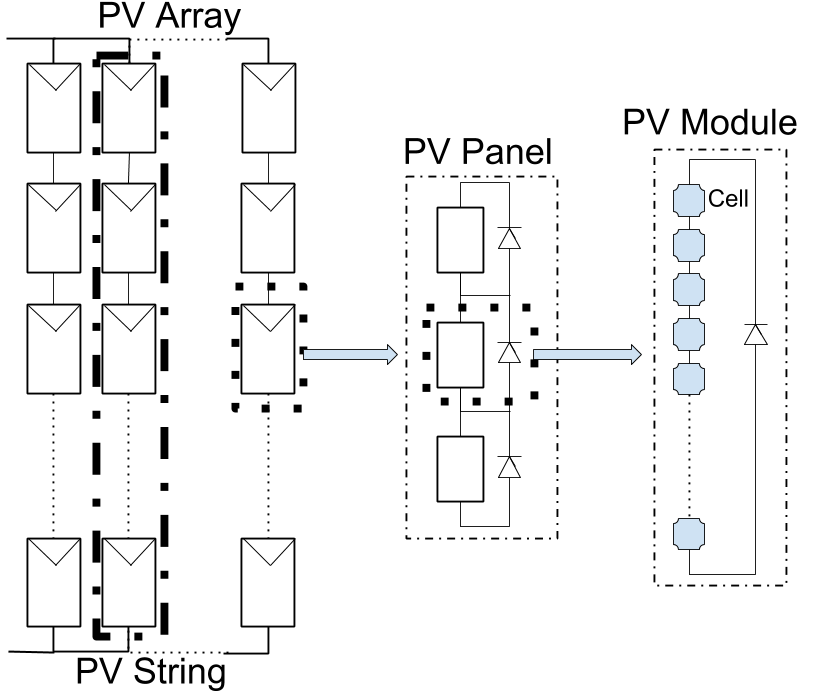
\includegraphics[width=\linewidth]{fig/module.png}}
\caption[]{PV array, string, module and panel}
\label{fig:array}
\end{figure}

\section{Feasibility Problem}
\subsection{Problem setting}
\subsection{Outline of the algorithm}
\subsection{Algorithm}
\section{Experiment Results}
\section{Conclusion}
The conclusion goes here.



\appendices
\section*{Acknowledgment}


The authors would like to thank...


% Can use something like this to put references on a page
% by themselves when using endfloat and the captionsoff option.
\section*{Temp}
It is well known that mismatch due to partial shading, soiling, or ageing causes significant losses
in the energy yield of photovoltaic (PV) systems [1,2]. Furthermore, mismatches may hinder operation
of maximum power point (MPP) tracking algorithms, especially if the power versus output voltage
characteristic becomes nonconvex [3]. It has also been shown that, even with commonly used bypass
diodes, mismatched cells may become reverse-biased and dissipate power, producing an undesired
cell temperature rise or hot spot [4,5]. This may lead to accelerated ageing and reduced reliability of
the PV system


\bibliographystyle{ieeetr}
\bibliography{library}


\end{document}


